\section{Introdução ao estudo das funções}

\subsection{Sistema cartesiano ortogonal de coordenadas}

O Sistema de coordenadas, mais conhecido como Plano Cartesiano, foi criado por 
René Descartes com o objetivo de localizar pontos. Ele é formado por dois eixos 
perpendiculares: um horizontal e outro vertical que se cruzam na origem das coordenadas. 
O eixo horizonal($0x$) é chamado de \textit{abscissa} e o vertical($0y$) chamado de ordenada. Os eixos 
são enumerados compreendendo o conjunto dos números reais. Observe a seguir a representação do 
Plano Cartesiano:

\begin{center}
  \begin{tikzpicture}
    \tkzInit[xmin=-5, xmax=5, xstep=1, ymin=-5, ymax=5, ystep=1]
    \tkzLabelX[orig=false]
    \tkzLabelY[orig=false]
    \tkzDrawXY
  \end{tikzpicture}
\end{center}

Para determinar as coordenadas do ponto \textit{P} da figura a seguir, traçamos por \textit{P} as 
perpendiculares ao eixo \textit{x} e ao eixo \textit{y}, obtendo, nesses eixos, dois números chamados 
de \textbf{abscissa} e \textbf{ordenada} do ponto \textit{P}, respectivamente.

\begin{center}
  \begin{tikzpicture}[scale=.7]
    \tkzInit[xmin=-5, xmax=5, xstep=1, ymin=-5, ymax=5, ystep=1]
    \tkzLabelX[orig=false]
    \tkzLabelY[orig=false]
    \tkzDrawXY
    \tkzDefPoint(5,4){P}
    \tkzDrawPoints(P)
    \tkzLabelPoint[right](P){$P$}
    \tkzPointShowCoord(P)
  \end{tikzpicture}
\end{center}

No exemplo, as \textbf{coordenadas} do ponto \textit{P} são 5 e 4. A \textbf{abscissa} é 5, e a \textbf{ordenada} é 4. 
Indicamos esse fato por $P(5,4)$.

A representação $(5,4)$ é chamada de ``\textbf{par ordenado} de abscissa 5 e ordenada 4''.

\begin{proposition}{Generalidades}{generalities}
  \begin{enumerate}
    \item Dois pares ordenados de números reais são iguais se, e somente se, suas abscissas são iguais e 
      suas ordenadas são iguais, isto é:

      \vspace{.2cm}
      $(a, b) = (c, d) \iff  a = c \text{ e } b = d$

      \vspace{.2cm}
      Por exemplo:

      \vspace{.2cm}
      $(a, 8) = (7, y) \iff a = 7 \text{ e } y = 8$

    \vspace{.2cm}
    \item Os eixos $0x$ e $0y$, chamados de \textbf{eixos coordenados}, separam o plano cartesiano em quatro 
      regiões denominadas \textbf{quadrantes}, que devem ser enumerados conforme a figura:

    \vspace{.2cm}
    \begin{center}
      \begin{tikzpicture}[scale=.7]
        \tkzInit[xmin=-10, xmax=10, xstep=1, ymin=-5, ymax=5, ystep=1]
        \tkzDrawXY[noticks]
        \tkzDefPoint(5,3){A}
        \tkzDefPoint(-5,3){B}
        \tkzDefPoint(-5,-3){C}
        \tkzDefPoint(5,-3){D}
        \tkzText[color = black](A){Primeiro Quadrante ($Q_1$)}
        \tkzText[color = black](B){Primeiro Quadrante ($Q_2$)}
        \tkzText[color = black](C){Primeiro Quadrante ($Q_3$)}
        \tkzText[color = black](D){Primeiro Quadrante ($Q_4$)}
      \end{tikzpicture}
    \end{center}

    \vspace{.2cm}
    \begin{tasks}(2)
      \task[] $P(a,b) \in Q_1 \iff a > 0 \text{ e } b > 0$
      \task[] $P(a,b) \in Q_2 \iff a < 0 \text{ e } b > 0$
      \task[] $P(a,b) \in Q_3 \iff a < 0 \text{ e } b < 0$
      \task[] $P(a,b) \in Q_4 \iff a > 0 \text{ e } b < 0$
    \end{tasks}

    \vspace{.2cm}
    Por exemplo:

    \vspace{.2cm}
    \begin{tasks}(2)
      \task[\#] $(4,2) \in Q_1$
      \task[\#] $(-\frac{1}{2},9) \in Q_2$ 
      \task[\#] $(-3,-5) \in Q_3$
      \task[\#] $(\frac{3}{2},-1) \in Q_4$
    \end{tasks}

    Os pontos dos eixos coordenados não pertencem a nenhum quadrante.

    \item Todo ponto de abscissa nula (igual a zero) pertence ao eixo $Oy$, e todo ponto de ordenada nula 
      (igual a zero) pertence ao eixo $0x$.

      \vspace{.2cm}
      Por exemplo:

      \vspace{.2cm}
      \begin{tasks}(2)
        \task[\#] $(0,-2) \in 0y$
        \task[\#] $(5,0) \in 0x$
      \end{tasks}
  \end{enumerate} 
\end{proposition}

\subsection{Exercícios Propostos}

\begin{enumerate}[label*=\protect\fbox{\arabic{enumi}}]
  \item Represente, no plano cartesiano, os seguintes pontos:
    \begin{tasks}(5)
      \task $A(4,2)$
      \task $B(2,4)$
      \task $C(-2,5)$
      \task $D(5,-2)$
      \task $E(-4,-1)$
      \task $F(-1,4)$
      \task $G(-6,0)$
      \task $H(0,-6)$
      \task $I(0,0)$
    \end{tasks}

  \item Para que valores reais de \textit{p} o ponto $A(p-7, \frac{4}{5})$ pertence ao eixo das ordenadas?
  \item Para que valores reais de \textit{k} o ponto $B(5k+15, 4k^2-36)$ pertence ao eixo das abscissas?
  \item Para que valores reais de r o ponto $C(\frac{2}{3}, r - 2)$ pertence ao $1^\circ$ quadrante?
  \item Determine os números reais \textit{a} e \textit{b} de modo que $(3a-2b, a+b) = (10, 11)$.
  \item O mapa ao lado está na escala $1 : 10.000$. Sabendo que o quadriculado é formado por quadradinhos de 1 cm de lado, 
    calcule a distância real entre os pontos da região representada, que correspondem no mapa a \textit{A} e \textit{B}.

    \begin{figure}[H]
      \centering
      
\includegraphics[width=.5\linewidth]{figures/1.png}
    \end{figure}

  \item Um ponto \textit{P} sobre a superfície da Terra é determinado por dois números chamados \textbf{latitude} e \textbf{longitude}. 
    A latitude de \textit{P} é a medida em grau do menor arco possível sobre um meridiano ligando o ponto \textit{P} à linha do equador. 
    A longitude de \textit{P} é a medida em grau do menor arco possível sobre um paralelo terrestre ligando o ponto \textit{P} ao meridiano 
    de Greenwich, e como negativas a latitude ao sul do equador e a longitude a oeste do meridiano de Greenwich. Um ponto sobre o equador tem 
    latitude $0^\circ$ e um ponto sobre o meridiano de Greenwich tem longitude $0^\circ$. Indica-se 
    o ponto \textit{P} pelo par ordenado $(x, y)$, sendo \textit{x} a latitude e \textit{y} a longitude. 

    O mapa abaixo é uma projeção plana da surpefície terrestre.

    \begin{figure}[H]
      \centering
      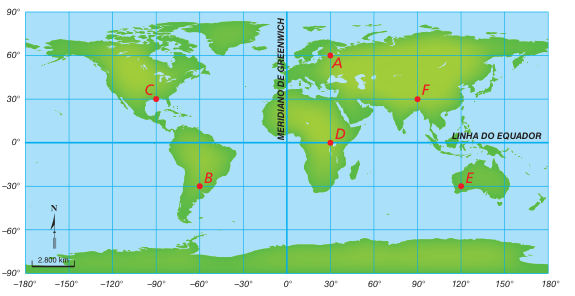
\includegraphics[width=1\linewidth]{figures/2.png}
    \end{figure}

    \begin{enumerate}[I]
      \item Entre os pontos assinalados em vermelho no mapa, determine as coordenadas do ponto:
        \begin{tasks}
          \task assinalado na região que corresponde à América do Sul.
          \task assinalado na região que corresponde à África.
          \task assinalado na região que corresponde à América do Norte.
          \task assinalado na região que corresponde à China.
          \task assinalado na região que corresponde à Europa.
          \task assinalado na região que corresponde à Austrália.
        \end{tasks}
      \item Em que continente está o ponto de latitude $60^\circ$ norte e longitude $120^\circ$ leste?
    \end{enumerate}
\end{enumerate}

